%Results:
%  - we took data and fit it to both full and naive models
%  - we got error bars
%  - within the error bars, both models kinda make sense.


\section{Results}
\label{sec:res}

\begin{figure*}[thb]%
\centering
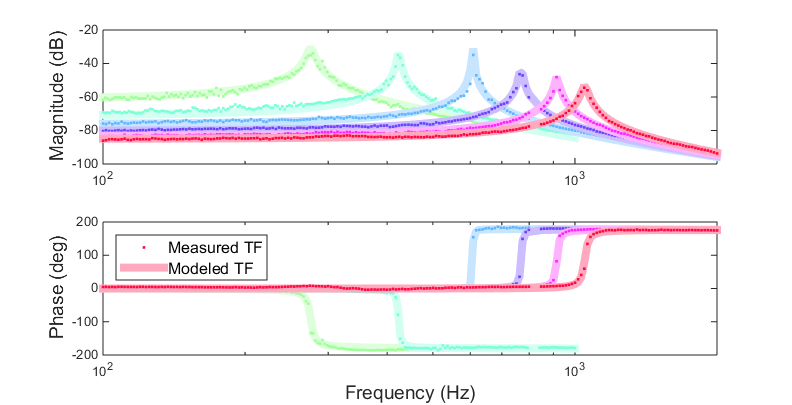
\includegraphics[width=.7\paperwidth]{figures/newOSfit.png}%
\caption{Data and modeled transfer function for a series of stable and unstable springs. The modeled transfer functions include the full coating and spot size correction, computed with the measured average absorption. Stable springs show a phase drop of 180 degrees at resonance, while unstable springs show a rise of 180 degrees.}%
\label{fig:springs}%
\end{figure*}
%\tcm{MUST BE REWRITTEN IN A POSITIVE WAY. WE have nice results to show not only problems. Because the previous version was literally depressing
%I remove it. Jim this is a section that you should have in your thesis, so you can plug it in and we will see how it flows.}
%\tcm{We also need to to say what function we are plotting...equation 1? 2? }

%At the beginning of the experiment, our goals were to measure and then accurately model a series of stable and unstable optical springs. During the course of the measurements, we saw a consistent trend towards instability; each measurement we took was more unstable than our model predicted it should be. We realized that this behavior was exactly what we would see from the photo-thermal effect. We made a new goal of measuring the effects of the photo-thermal absorption.

Using the setup described in the previous section, we locked the cavity using a PDH error signal from the sub-carrier, feeding back to the laser frequency actuator and, at low frequencies, the heavy input coupler position. In this configuration we fine-tuned the optical spring parameters (carrier and sub-carrier offset and power) and 
measured the PDH control loop open loop transfer function. Dividing out the known PDH loop sensing and actuation function gives us the closed loop transfer functions of the optical springs (figure \ref{fig:springs}). While we demonstrated stable and unstable dual-carrier optical springs, these measurements revealed a significantly smaller phase margin of the optical spring than expected based on equation \ref{eqn:TFloop}, suggesting the presence of a non-radiation-pressure feed-back path.

At a few ppm, the absorption $A$ of the mirrors has a very small effect on the cavity finesse and no significant impact on the total transmitted power. However, this small amount of absorption still causes local heating of the optic, driving fluctuations in the surface position of the optic, and thus the cavity length, via the photo-thermal effect. If this is the dominant effect, we should be able to include the photo-thermal effect in our model and fit the model to the data, using the absorption as the free parameter. Given a set of optical spring measurements done under similar conditions, we would then expect to find a consistent absorption coefficient across measurements.

%\begin{table*}[t]
%\small
%\begin{tabular}{| l || c | c | c | c | c | c | c |}
%\hline 
%Run & 14 & 10 & 9 & 16 & 17 & 18 & 19 \\
	%\hline
	%\hline
%$f_{res}$ [Hz]& $386 \pm 3$& $423 \pm 2$& $432 \pm 2$& $609 \pm 5$& $772 \pm 6$& $919 \pm 7$& $1054 \pm 8$\\
%$P_{tc}$ [mW]& $44.1 \pm 0.9$& $45.3 \pm 0.9$& $45.3 \pm 0.9$& $49.3 \pm 1.0$& $54.0 \pm 1.1$& $59.8 \pm 1.2$& $67.2 \pm 1.3$\\
%$P_{ts}$ [mW]& $63.9 \pm 1.3$& $73.2 \pm 1.5$& $73.2 \pm 1.5$& $62.6 \pm 1.3$& $62.1 \pm 1.2$& $62.3 \pm 1.2$& $61.8 \pm 1.2$\\
%$df$ [KHz]& $320 \pm 5$& $320 \pm 5$& $320 \pm 5$& $300 \pm 5$& $280 \pm 5$& $260 \pm 5$& $240 \pm 5$\\
%\hline$P_{ic}$ [mW]& $225 \pm 16$& $239 \pm 17$& $239 \pm 17$& $227 \pm 17$& $225 \pm 17$& $225 \pm 17$& $223 \pm 17$\\
%$P_{is}$ [mW]& $69.5 \pm 1.6$& $78.3 \pm 1.7$& $78.2 \pm 1.6$& $67.6 \pm 1.6$& $66.5 \pm 1.6$& $66.2 \pm 1.5$& $65.6 \pm 1.6$\\
%$\delta f_c$ [KHz]& $284 \pm 8$& $290 \pm 7$& $290 \pm 7$& $267 \pm 8$& $250 \pm 8$& $233 \pm 8$& $213 \pm 9$\\
%$\delta f_s$ [KHz]& $-36 \pm 5$& $-30 \pm 4$& $-30 \pm 4$& $-33 \pm 6$& $-30 \pm 6$& $-27 \pm 6$& $-27 \pm 7$\\
%\hline$A$ [ppm]& $2.9 \pm 2.16$& $2.7 \pm 2.20$& $2.9 \pm 1.80$& $2.8 \pm 1.77$& $2.5 \pm 1.31$& $2.5 \pm 1.08$& $2.7 \pm 0.96$\\
%$\phi$ [mRad]& $-15 \pm 11$& $-15 \pm 12$& $-17 \pm 10$& $-25 \pm 15$& $-29 \pm 15$& $-36 \pm 15$& $-46 \pm 16$\\
%
%
%\hline
%
%
%\end{tabular}	
%\normalsize
%\caption{Measured values [$f_{res}$, $P_{tc}$, $P_{ts}$, $df$], translated to optical spring parameters [$P_{ic}$, $P_{is}$, $\delta f_c$, $\delta f_s$] and the calculated absorption coefficient $A$. \tcb{sort by fres}}
	%\label{tab:springs}
	%
%\end{table*}

\subsection{Analysis}

For each measured optical spring transfer function we record the carrier and subcarrier transmitted powers, $P_{tc}$ and $P_{ts}$, the optical spring resonance frequency $f_{res}$, and the difference between the carrier and subcarrier detunings $df_c-df_s$, which is set by the function generator frequency.   

%Using these values we can accurately determine the parameters [$P_{is}$,$P_{ic}$, $df_c$,$df_s$], namely
%the power coupling into the cavity and the detuning for both the carrier and the subcarrier at the time of measurement. %\tcr{This is useful because we had a little bit of alignment drift during the course of the experiment.}
%Equation \ref{eqn:TFloop} allows us to convert these four parameters into an optical spring transfer function.

We can then fit the data $d$ using a model $m$, which includes the photo-thermal effect. In particular we fit the ratio $d/m$ using a least-squares fit to minimize $E$, the error.
\begin{equation}
E=\Sigma \left|\frac{d}{m}-1\right|^2 
\end{equation}

We fit for a small magnitude offset, the subcarrier detuning $df_s$, and the absorption $A$. We assess the fitting errors by modeling the noise in each frequency bin of the transfer function measurement, and propagating this noise through the fit. Four of the optical spring transfer functions  had a measurement noise of a little less than $1~{\rm dB}$, while the optical springs at $276~{\rm Hz}$ and $422~{\rm Hz}$ had a significantly higher noise of about $3~{\rm dB}$. We think this noise is dominated by intra-cavity power fluctuations, most likely due to angular fluctuations.

The remaining parameters (cavity transmitted powers and carrier-sub-carrier frequency spacing) we treat as systematic errors. We propagated their measurment errors through the fit. We used a $2\%$ measurement error for the power measurements and  a $1~{\rm kHz}$ error for the frequency separation.




%\begin{eqnarray}
%E=\Sigma w|d-m|^2 \hspace{5pt} w = m^{-2}\\
%\frac{\partial E}{\partial p_i} = 0\\
%\Sigma w(d-m) \frac{\partial m}{\partial p_i} = 0
%\label{eq:dEdP}
%\end{eqnarray}
%We are evaluating two different models: 
	%(i) a naive model, with a simple $1/f$ behavior representative of a single slab of fused silica (equation \ref{eq:simple}), and
  %(ii) a combined model, adding both coating and diffusion effects to the naive model (equations \ref{eq:Cerdonio} and \ref{eq:dphic2}).

%We can calculate the error for each fitted parameter based on the noise in the transfer function and the discrepancy between the best fit model and the data. 

%We determine the change in the model $m$ with respect to the six parameters of the system (three measured and three fitted)
%\begin{equation}
%M_i' = \frac{\partial m}{\partial p_i}
%\label{eq:}
%\end{equation}

%We construct a vector $\epsilon$ to contian the error on each of the six parameters. Then we assert that the noise $n$ seen during the data recording were likely caused by the fluctation of some or all of the parameters. We combine that with the mismatch between model and data to arrive at the uncertainty in the different parameters.

%\begin{eqnarray}
%M'\epsilon = (n+d-m);\\
%M'^\dagger M'\epsilon = M^\dagger(n+d-m);\\
%\epsilon = (M'^\dagger M')^{-1}M^\dagger(n+d-m);
%\label{eq:epsilonDef}
%\end{eqnarray}
%\begin{equation}
%\epsilon = (M'^\dagger M')^{-1}M^\dagger(n+d-m);
%\label{eq:epsilon}
%\end{equation}

%This gives us the uncertainty in absorption $e_{A}$ due to the fluctuations of other parameters during measurements.


%$M'$ is an $a\times b$ matrix where a is the number of frequency points in the transfer function and b is the number of parameters used in total: three fixed parameters and three fitted parameters. We determine $M'$ by taking the partial derivative of the model $M$ at each frequency point with respect to each parameter $p_i$. $M'^\dagger$ is the transposed complex conjugate of $M'$.

%We calculate the error in the absorption $A$ by propagating the individual measurement errors through the analysis, refitting the absorption $A$, and adding all errors in quadrature. Errors for $P_{ts}$ and $P_{tc}$ are $2\%$ of the measured value, accounting for oscilloscope inaccuracies, fluctuations over the course of the measurement, and DC offsets of the photodiodes.  Error for the frequency offset are a flat 5KHz; we have determined that the frequency output is accurate to 1 or 2 KHz, but we did not always place the dial precisely during measurements. $f_{res}$ can be determined to about 1 Hz, limited by how well we can fit the data given the finite frequency spacing. It is this error on the resonance frequency that dominates the total measurement error.

After determining the absorption $A$ for each optical spring transfer function measurement, we can take a statistical-error-weighted average to arrive at the most probable absorption coefficient for the mirror.  For the full photo-thermal model we measure a consistent absorption of  $2.60\pm0.08$ ppm ($\pm 0.06$ ppm statistical,  $\pm 0.05$ ppm systematic) (see figure \ref{fig:abs}). The naive $1/f$ model yields an absorption of $3.27\pm0.10$ ppm ($\pm 0.08$ ppm statistical,  $\pm 0.06$ ppm systematic).  The detailed model with coating and spot size corrections is slightly preferred by the data over the naive $1/f$ model, i.e. the result is more consistent with the same absorption at all frequencies. However the errors in our mesurement are too large to make this statement with any sigificant certainty.

%\begin{eqnarray}
%A_ = \frac{\Sigma\left(A\epsilon_{A}^{-2}\right)}{\Sigma\left(\epsilon_{A}^{-2}\right)}
%\hspace{20pt}
%\sigma_{ABS} = \sqrt{\frac{1}{\Sigma\left(\epsilon_{Ai}^{-2}\right)}};
%\label{eq:weighting}
%\end{eqnarray}


Since this measurement is based on the missing optical spring phase on resonance, we can also express the result as extra phase. Near the resonance the optical spring constant is close to real, while the photo-thermal effect is almost purely imaginary. Thus we approximately find for the extra phase $\phi$
\begin{equation}
\phi =  2 m \Omega^2 \frac{c}{2} \frac{\bar{\alpha}}{\Omega \rho C \w^2 \pi} A I_{\rm corr}
\approx 0.4^{\circ} \frac{A I_{\rm corr}}{1~{\rm ppm}} \frac{f}{1~{\rm kHz}} 
\label{eq:phase}
\end{equation}
Here the leading factor of two accounts for the two mirrors, $I_{\rm corr}$ is the real part of the total correction factor plotted in figure \ref{fig:PTcorr}, and we used the material parameters for fused silica (see table \ref{SiO2}).  
Figure \ref{fig:phi} shows the measured extra phase on resonance, together with the prediction from the photo-thermal feed-back with the best-fit absorption. The figure also shows the expected phase due to the dual-carrier optical spring, as well as the total phase of the complete model. Finally it is worth mentioning that this is a remarkably precise way to measure the phase of the open loop transfer function - the  error bars in figure \ref{fig:phi} are as small as $0.04^{\circ}$.






%
%Since the main effect of the thermo-optic feed-back is a change in the optical spring phase margin, we can alternatively express our measurment as additional phase required to fit the data. 
%{\tcr{rewritten till here}}
%We can use this value to create a model for $\phi_{pt}$ as a function of $f_{res}$ by varying $df_c$.  We can then compare this model to the measured $\phi_{pt}$.
%
%We can see in Figure \ref{fig:phi} that there is excellent agreement between the full model and the measured loss angles $\phi_{pt}$.  
%
%From this point, we calculate the quality factor $Q$ and total (photothermal effect and optical spring damping) loss angle $\phi_{pt+os}$ for each model ($Q = \frac{f_{res}}{\mbox{FWHM}} = \frac{1}{\phi_{pt+os}}$).  Using the fitted model rather than data is a much more accurate method of determining the optical spring $Q$ because the measured data is limited in frequency resolution, making it difficult to determine the full-width-half-max (FWHM) accurately.  Using the models that fit the data closely, we can increase the resolution and get a reliable measure of the Q  (and thus $\phi_{pt+os}$).
%
%We can similarly calculate the loss $\phi_{os}$ for an optical spring with the same parameters but no absorption (and thus no photo-thermal effect).  Because the effect is purely imaginary and the real part of the transfer function is consistent, the phases can be subtracted. We arrive at $\phi_{pt} = \phi_{pt+os} - \phi_{os}$, the loss due to the photo-thermal effect (see figure \ref{fig:phi}).  
%
%
%%For each one of these errors, we add or subtract the error from the measured value in one of the parameters, then recompute $\phi_{pt}$ and $A$. We find the difference between upper and lower propagated errors for each parameter, add them in quadrature, and finally divide by 2 to get the error bars for $\phi_{pt}$ and $A$.
%
%Once we have calculated $A$ for a number of measurements, we can take an error-weighted average to arrive at the most probable absorption coefficient for the mirror.  We can use this value to create a model for $\phi_{pt}$ as a function of $f_{res}$ by varying $df_c$.  We can then compare this model to the measured $\phi_{pt}$.
%
%We can see in Figure \ref{fig:phi} that there is excellent agreement between the full model and the measured loss angles $\phi_{pt}$.  We measure a consistent absorption of about  $2.7 \pm 0.06$ ppm (see figure \ref{fig:abs}). The calculated reduced chi-squared is about 0.32, indicating that our statistical error is much smaller than the systematic error. The agreement between the data and the naive model is worse, yielding a reduced chi-squared of about 4.6 for an absorption of about $6.49 \pm 0.21$ ppm.

\begin{figure}[htb]%
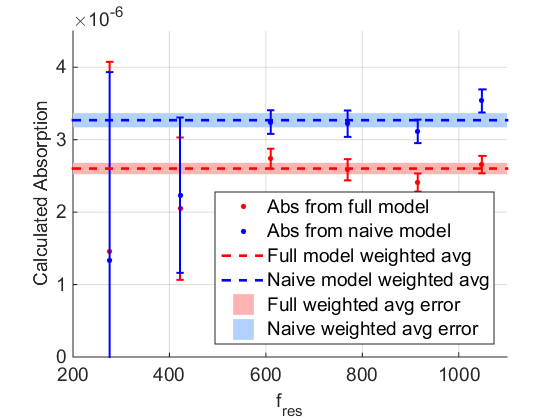
\includegraphics[width=\columnwidth]{figures/newABS.png}%
\caption{Absorption fit for naive and full models. The full model absorption is consistent with a constant absorption of  $2.60\pm0.08$ ppm. The naive $1/f$ model predicts $3.27\pm0.10$ ppm. The transfer function data for the lowest two resonant frequencies was significantly noisier. Also, at lower frequencies the photo-thermal  effect has a smaller effect on the total optical spring. Both effects result in the larger error bars at low frequencies.}
\label{fig:abs}%
\end{figure}

\begin{figure}[htb]%
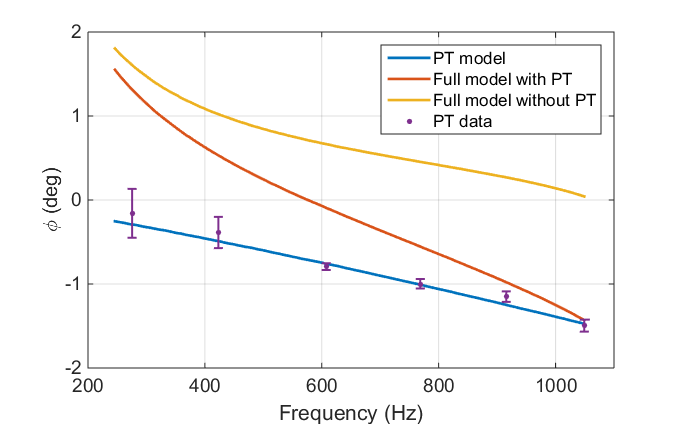
\includegraphics[width=\columnwidth]{figures/newPhi.png}%
\caption{Feedback phase in the system due to the optical spring and photo-thermal effect. The measured extra phase is consistent with $2.60$ ppm of absorption. The error bars are as small as $\pm 0.04^{\circ}$, a remarkable precision for an open loop transfer function phase measurement.
}
\label{fig:phi}%
\end{figure}

%\begin{figure}[htb]%
%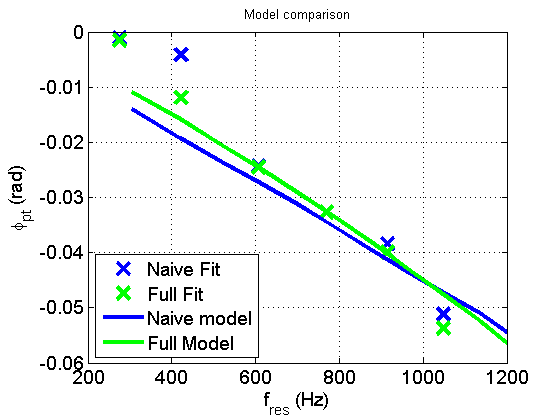
\includegraphics[width=\columnwidth]{figures/phi.png}%
%\caption{Data and model for the loss angle $\phi$ for the full model.}%
%\label{fig:phi}%
%\end{figure}



%We can use the fact that the phase of the optical spring is very closely tied to its stability to measure the absorption $A$ of the mirrors very accurately. As the optical spring system approaches instability, its quality factor (Q) rapidly increases. By measuring the Q of the optical spring and comparing to the model which does not include the photo-thermal effect, we can determine the phase of the actuation function and thus the absorption of the optic to high accuracy (see Figure \ref{fig:absvsq}).  We note that optical springs closer to the stability critical point (resonant frequency of about 500 Hz in our measurements) have a large (positive or negative) slope 
%
%The six measurements given in table \ref{tab:springs} are shown in figure \ref{fig:springs}. These are measurements of the locked trap cavity open loop transfer function. In this case we drive the locked servo, which in turn actuates on the laser PZT and input mirror position, in high and low frequency ranges, respectively. We measure the signal immediately before the servo. From figure \ref{fig:springs}, we can identify that three of the configurations are stable (with phase dropping 180 degrees at the resonant frequency) and three are unstable (with phase rising 180 degrees instead).
%
%
%\begin{figure}[ht]
%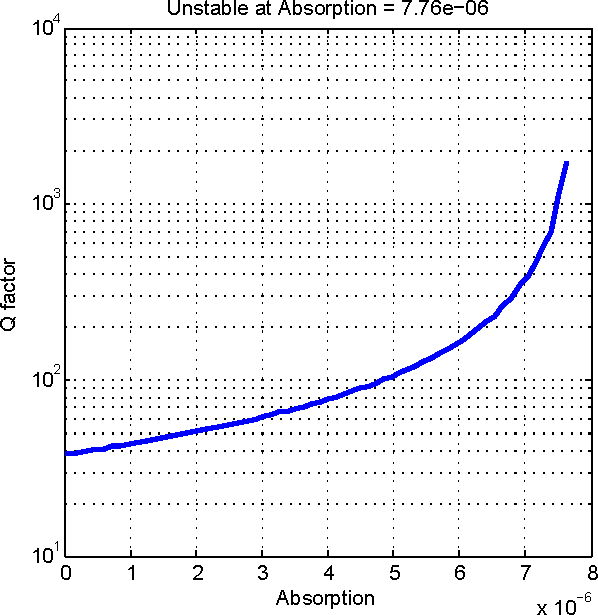
\includegraphics[width=.8\columnwidth]{figures/AbsVsQ.png}%
%\caption{Model for optical spring Q as a function of absorption. Given a set of input parameters for an optical spring, the Q will be directly related to the absorption coefficient.  Optical springs that are closer to the stability critical point have a higher absolute slope, which means that we can measure the absorption more precisely.}%
%\label{fig:absvsq}%
%\end{figure}
%
%\newpage
%
%\begin{figure}[ht]
%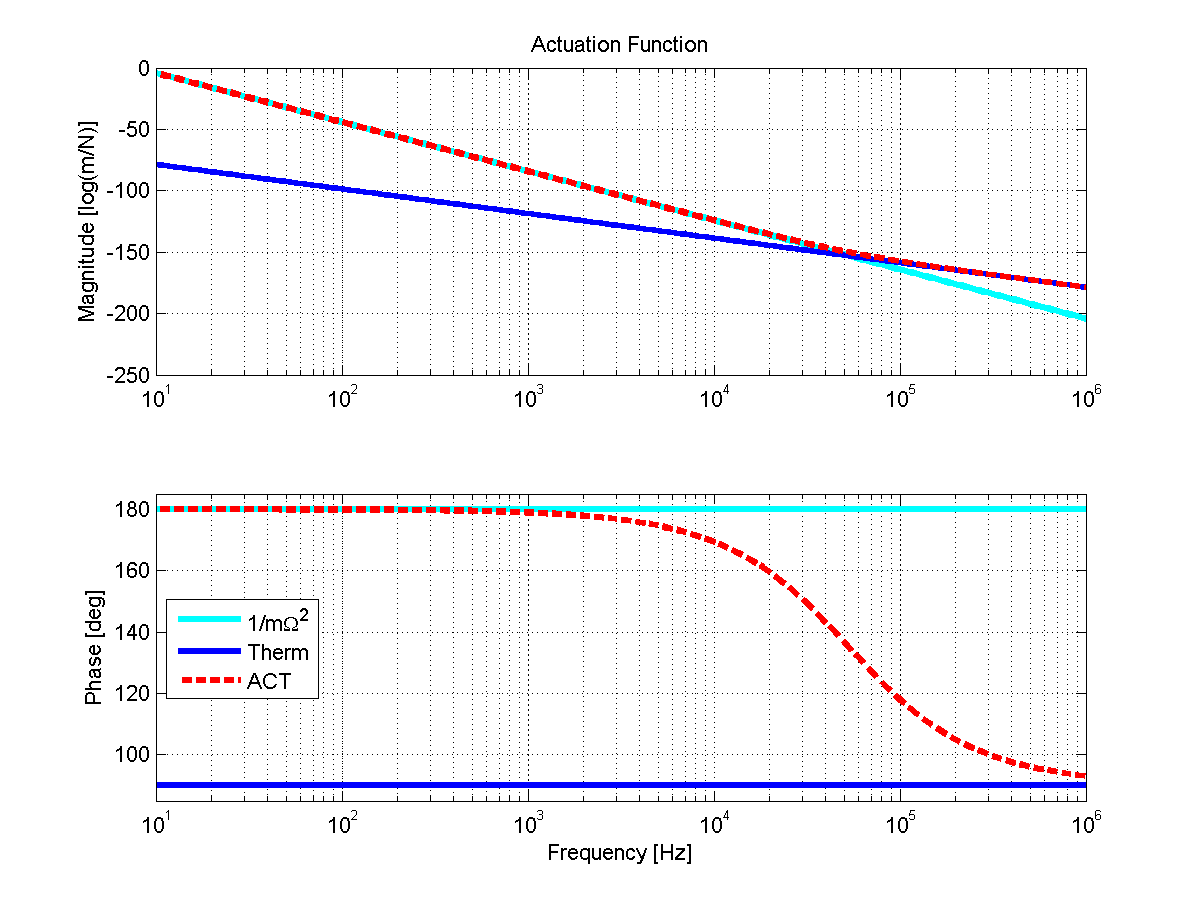
\includegraphics[width=.8\columnwidth]{figures/ACT.png}%
%\caption{Actuation function for small mass. As the frequency increases, the phase contribution from the photo-thermal effect becomes significant.\tcb{should go in intro}}%
%\label{fig:act}%
%\end{figure}
%
%
%Using this method, we can measure the absorption of the mirrors to be $6 \pm x$ ppm \tcm{need to verify this number}, which is \tcb{more accurate/as accurate/cooler} than previous measurements.

%A frequency-dependent thermal expansion of the optic can accurately reproduce the stability behavior observed \cite{BallmerThesis}. This effect is due to absorption of intra-cavity light (about 5 ppm) on the surface of the optic which causes local heating following the thermal diffusion law:
%
%\begin{equation}
%C \rho \frac{\partial T}{\partial t} = \kappa \nabla^2 T
%\label{eq:fourier}
%\end{equation}
%
%Where $C$ is the heat capacity, $\rho$ is the density, and $\kappa$ is the thermal diffusivity.  The heated areas expand at a rate governed by thermal expansion coefficient $\alpha$; because this heating is local, the only possible direction of expanion is the optical axis, towards the center of the cavity. This introduces a factor of $\eta$, Poisson's ratio.
%
%
%\begin{equation}
%\delta z = \alpha(1+\eta) \int_0^\infty{T dz}
%\label{eq:deltaz}
%\end{equation}
%
%The low frequency behavior of this effect is easy to understand and model.  However, when the cavity length is fluctuating, there is frequency dependent behavior that is interesting.
%
%\begin{eqnarray}
%\frac{\delta z}{F_{ext}} = \imath\frac{c}{2 C \rho} \frac{1+\eta}{\pi w^2} \frac{2 \alpha A}{\Omega}\\
%\frac{\delta z}{\delta L} = -m\Omega^2\imath\frac{c}{2 C \rho} \frac{1+\eta}{\pi w^2} \frac{2 \alpha A}{\Omega}
%\label{eq:}
%\end{eqnarray}




%We found a range of stable and unstable springs and we can model the behavior well (see figure \ref{fig:springs}). The largest uncertainty in the measurement was the intra-cavity power.  This is affected by mode matching, cavity alignment, cavity finesse, and input power. As we mentioned earlier, we were very careful to maintain the coatings of the mirror during the cavity construction process.  \tcb{We do have a question about whether the cavity finesse is affected by mode matching.}  We know the input power and the power fluctuation from the laser data sheet \tcb{(and we can predict how much intensity noise the Subcarrier Servo introduces)}. This leaves one big question: the cavity alignment. Because of our digital system design, we do not have any feedback at very low frequencies, instead relying on the pendulum behavior of the suspension.  This can cause trouble with drifting, which we expect is the single largest contributor to variances in the intra-cavity power.
%
%Intensity fluctuations also couple to cavity length via heating of the surface of the mirrors. It's a lot weaker than other noise sources at low frequencies, but only drops as $1/f$, compared to $1/f^2$ for most other noise sources. With this coupling (on both mirrors) and an assumed absorption of 5 ppm, the data can be fairly well explained\cite{BallmerThesis}.



%From our model, we can estimate the length of the stability region of a particular optical trap based on the detuning and power parameters. For the parameters \tcb{$\delta_{C} = 285 \mbox{KHz}$, $\delta_S = -35\mbox{KHz}$, and $P_C/P_S = 3.50$} we find a stable region of \tcb{27 \mbox{pm}}. Thus, if we can lower our RMS length noise to about \tcb{14 pm} we could feasibly turn off or significantly reduce active feedback.
%
%Figure \ref{fig:trapnoise} shows the various noise sources in our experiment. \tcb{Once we get the final plot, we should describe interesting things in it.} At high frequency, our current limitation is the laser frequency noise.  At lower frequencies, we have laser intensity noise and seismic motion to contend with.

%It looks like the intensity noise contribution is much higher than it is plotted on the graph.
%
%The behavior of the intensity noise at 500 Hz could use some explaining. Is this because we are dividing by the closed loop tf?
%
%What do we have in terms of optical trap for this measurement?
%
%Subcarrier: -50KHz, Carrier: 280KHz, Transmitted power ratio C/SC 0.720
%\tcb{We need the updated plot!}
%\tcb{Using this noise measurement, we can see that by doing X, Y, and maybe Z, we could feasibly run the trap with NO active feedback to the cavity length.}

%\begin{figure}[htb]
%\centering
  %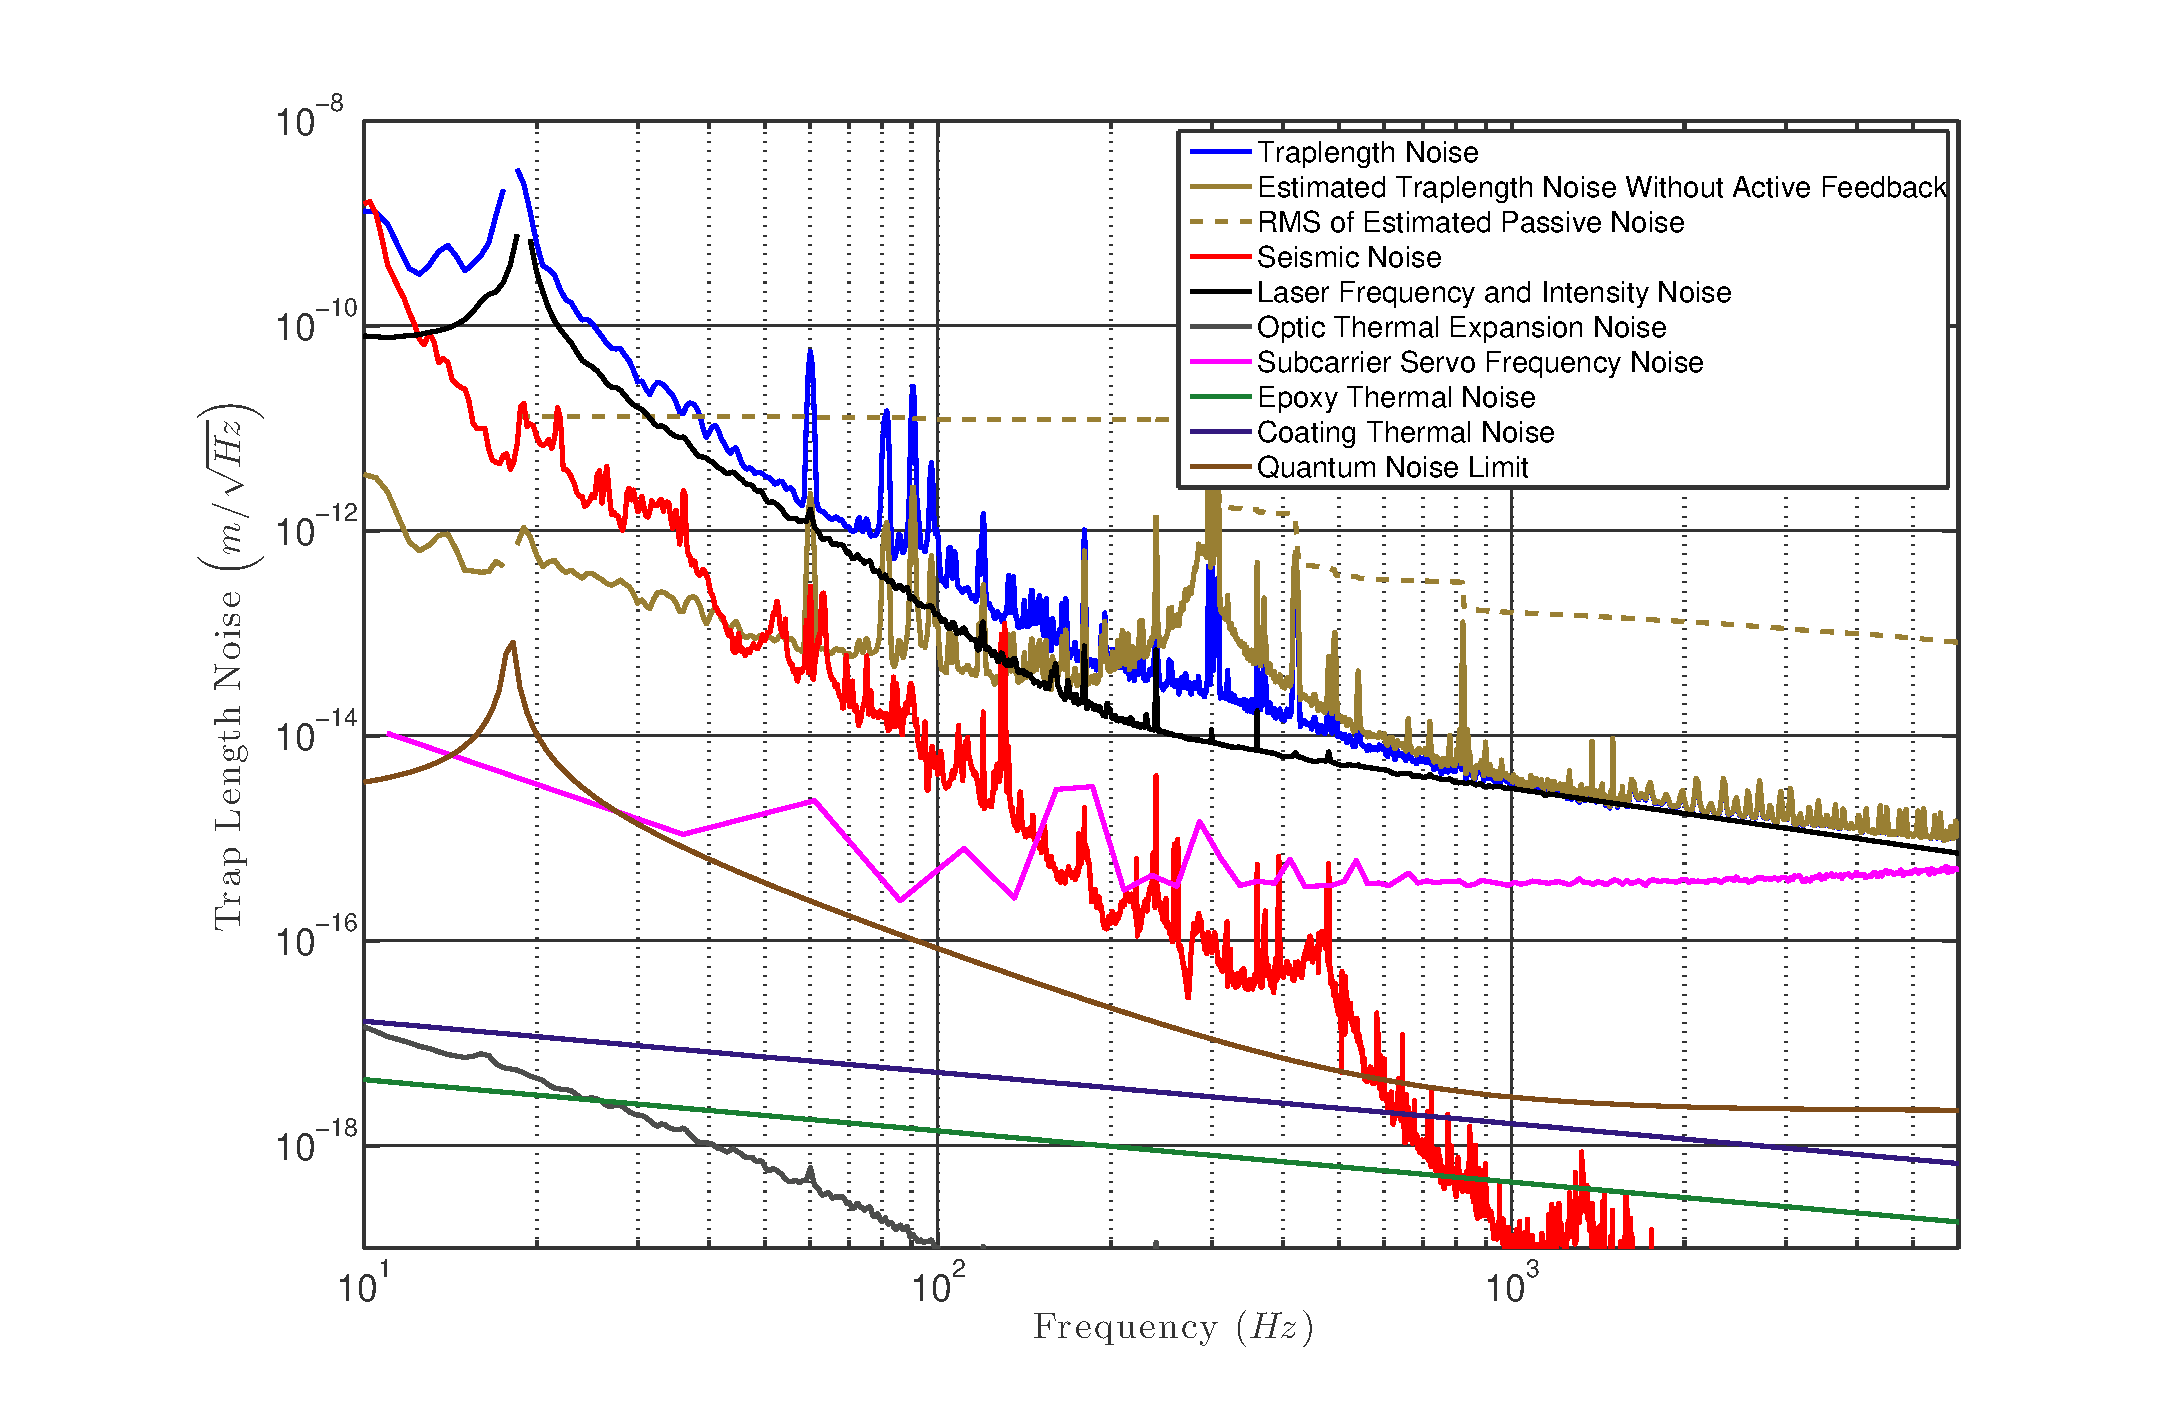
\includegraphics[width=0.8\columnwidth]{figures/trapnoise}
  %\caption{This is the noise budget for the experiment. SC: -50 C: 280
    %TPR .720.
    %\tcb{Updated plot (14.08.02). We may want to have a separate plot
    %for the estimated noise without active feedback.}
    %}
  %\label{fig:trapnoise}
%\end{figure}

\section{Stable single-carrier optical spring}
\label{sec:SCs}
In the experiment at hand the photo-thermal feed-back always pushed the optical spring resonance closer to instability.
Perhaps the most interesting question is whether we can change the sign of this feed-back path and exploit it to stabilize an otherwise unstable optical spring. It was pointed out in \cite{PhysRevD.91.023010} that this naturally occurs above about $100~{\rm kHz}$ for a regular dielectric coating. 
At those frequencies the thermal diffusion length only affects the first few layers of the coating, which affect the overall coating reflected phase differently than the rest of the coating.
However it is actually quite simple to get this sign inversion to occur at a much lower frequency. Increasing the thickness of the inital half-wavelength $SiO_2$ layer - but keeping it an odd multiple of half the wavelength - will boost the effect from the first layer, thus lowering the frequency at which this sign inversion occurs. Indeed this effect can be strong enough that the damping effect from the sub-carrier is not needed to generate a stable optical spring. To illustrate this, figure \ref{fig:SCsprings} shows a set of six optical springs with parameters identical to the ones shown in figure \ref{fig:springs}, except that we set the sub-carrier power to zero (i.e. they are single-carrier optical springs), and we increased the first $SiO_2$ coating layer from $0.5$ wavelength to $20.5$ wavelength.

Such a modified coating would thus allow detuned self-locking  of an optical cavity, using just one laser frequency. It does rely on a small amount (order 1 ppm) of optical absorption in the coating, but this level of absorption is often unavoidable anyway, and does not prevent high-finesse cavities. 
\begin{figure*}[thb]
\centering
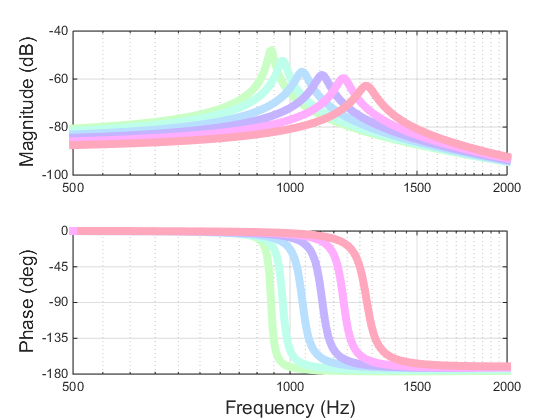
\includegraphics[width=.7\paperwidth]{figures/singleCarrierSprings}
\caption{Stable single-carrier optical springs (no sub-carrier) with modified coating - the first coating layer is $20.5$ wavelength thick. See text for details. The six traces otherwise have the same parameters as the best-fit optical springs in figure \ref{fig:springs}. }
\label{fig:SCsprings}
\end{figure*}








\section{Conclusions}
We observed photo-thermal feedback in an experimental optical spring setup for a 0.4 gram mirror. We made measurements for a range of optical spring resonant frequencies, and used a least squares fit to calculate the absorption. The data is consistent with the predictions of the complete model presented in Section \ref{sec:PTE}, but only sligthly prefers it over a simple model that ignores any heat diffusion in the coating and transverse to the optical axis. We also show that a small modification of the first layer of the high-reflectivity coating would be enough to reverse the sign of the photo-thermal feed-back, to the extent that a single-carrier, dynamically and statically stable optical spring becomes feasable.

%We presented a model for a complete photo-thermal effect in a cavity optical springs. This model included radial diffusion behavior, coating expansion, and bulk expansion. We described the optical trap experiment at Syracuse University as it relates to the creation of optical springs influenced by the photo-thermal effect. We measured stable and unstable optical springs, which showed more instability than the basic optical spring model predicted. We used a naive model and a complete model of the photo-thermal effect to fit the data. We found excellent agreement between the measured data and the complete photo-thermal effect model.

Repeating the presented measurement with a folding mirror in a cavity should also allow us to confirm the predicted enhancement of thermal noise for folding mirrors \cite{PhysRevD.90.042001} . This noise will affect any gravitational-wave interferometer design making use of folding mirrors in the arm cavities \cite{Ballmer13}.



%This also has implications for the angular trap we are currently developing. We plan to have a folded cavity which will have a standing wave interference pattern on the small mirror. Choosing a large angle for the folded side cavity reduces the peak separation of the interference pattern. This peak separation determines the characteristic time for the front surface to reach thermal equilibrium. If this time is comparable to or greater than than the beam fluctuation period, there can be extra thermal expansion in the regions with the interference peaks. This effect adds coherently, causing the amplification of the photo-thermal effect above a cutoff frequency.

%We also plan to use a lower resonant frequency, which will also reduce the magnitude of the photo-thermal effect.


%We expect this effect will become increasingly important as intra-cavity power increases and optical springs are considered in the new generation of advanced gravitational-wave detectors.

%
%We set optical springs near the critical point between stable and unstable, then used the quality factor of the spring to determine the absorption of the mirrors.  We were able to measure the photo-thermal effect to ??? precision. The measured behavior matched the predictions of the low ($f< 2$ KHz) frequency regime of the photo-thermal effect.
%
%We don't expect much in the way of exciting deviations from the Gaussian 0,0 behavior in the angular trap.

%What have we learned from building the longitudinal trap?
%\begin{itemize}
	%\item We are intensity limited in the 10-200ish HZ range, so the ISS could potentially help.
	%\item PMC would be nice, but we have to make it work with the laser drive, adding a potentially fragile loop in the middle of everything.
	%\item The current FSS is downright incompatable with our trap locking scheme.  It might be possible to make an adder of sorts if we need it. we are dominated at high frequency by laser frequency noise
	%\item Position and laser feedback is a reasonable way to get optical spring behavior
	%\item seismic isolation is really important below 20 HZ... we may have to improve it
%\end{itemize}
%plan: 
%\begin{itemize}
	%\item lock main cavity on subcarrier using position and laser feedback
	%\item lock side cavity on subcarrier, using yaw feedback
	%\item gradually ramp up carrier light into both using waveplate between PBS0's
%\end{itemize}
%
%What are the big challenges?
%
%\begin{itemize}
	%\item design and build the new layout
%\end{itemize}

\input{tableSiO2Ta2O5}

\section{Acknowledgments}

This work was supported by the National Science Foundation grant PHY-1068809. The authors used computer resources supported by NSF grants PHY-1040231, PHY-1104371, and PHY-0600953.
This document has been assigned the LIGO Laboratory document number LIGO-P1500003.
